\documentclass{mydoc}
\usepackage{dirtree}
\usepackage{booktabs}

\title{\dabiaosong 区块链作业---Merkle Tree 实现与优化}
\author{张丘洋 D202081011}

\begin{document}

\maketitle

\section{Merkle Tree 简介}

Merkle Tree(默克尔树) 是一种哈希树,其每个叶子节点均以数据块的哈希作为标签,
而除了叶节点以外的中间节点则以其子节点标签的加密哈希作为标签。哈希树能够高效、
安全地验证大型数据结构的内容,是哈希链的一种推广形式。

Merkle Tree 的示意图如图 \ref{fig:merkle-tree} 所示。

\begin{figure}[htbp]
  \centering
  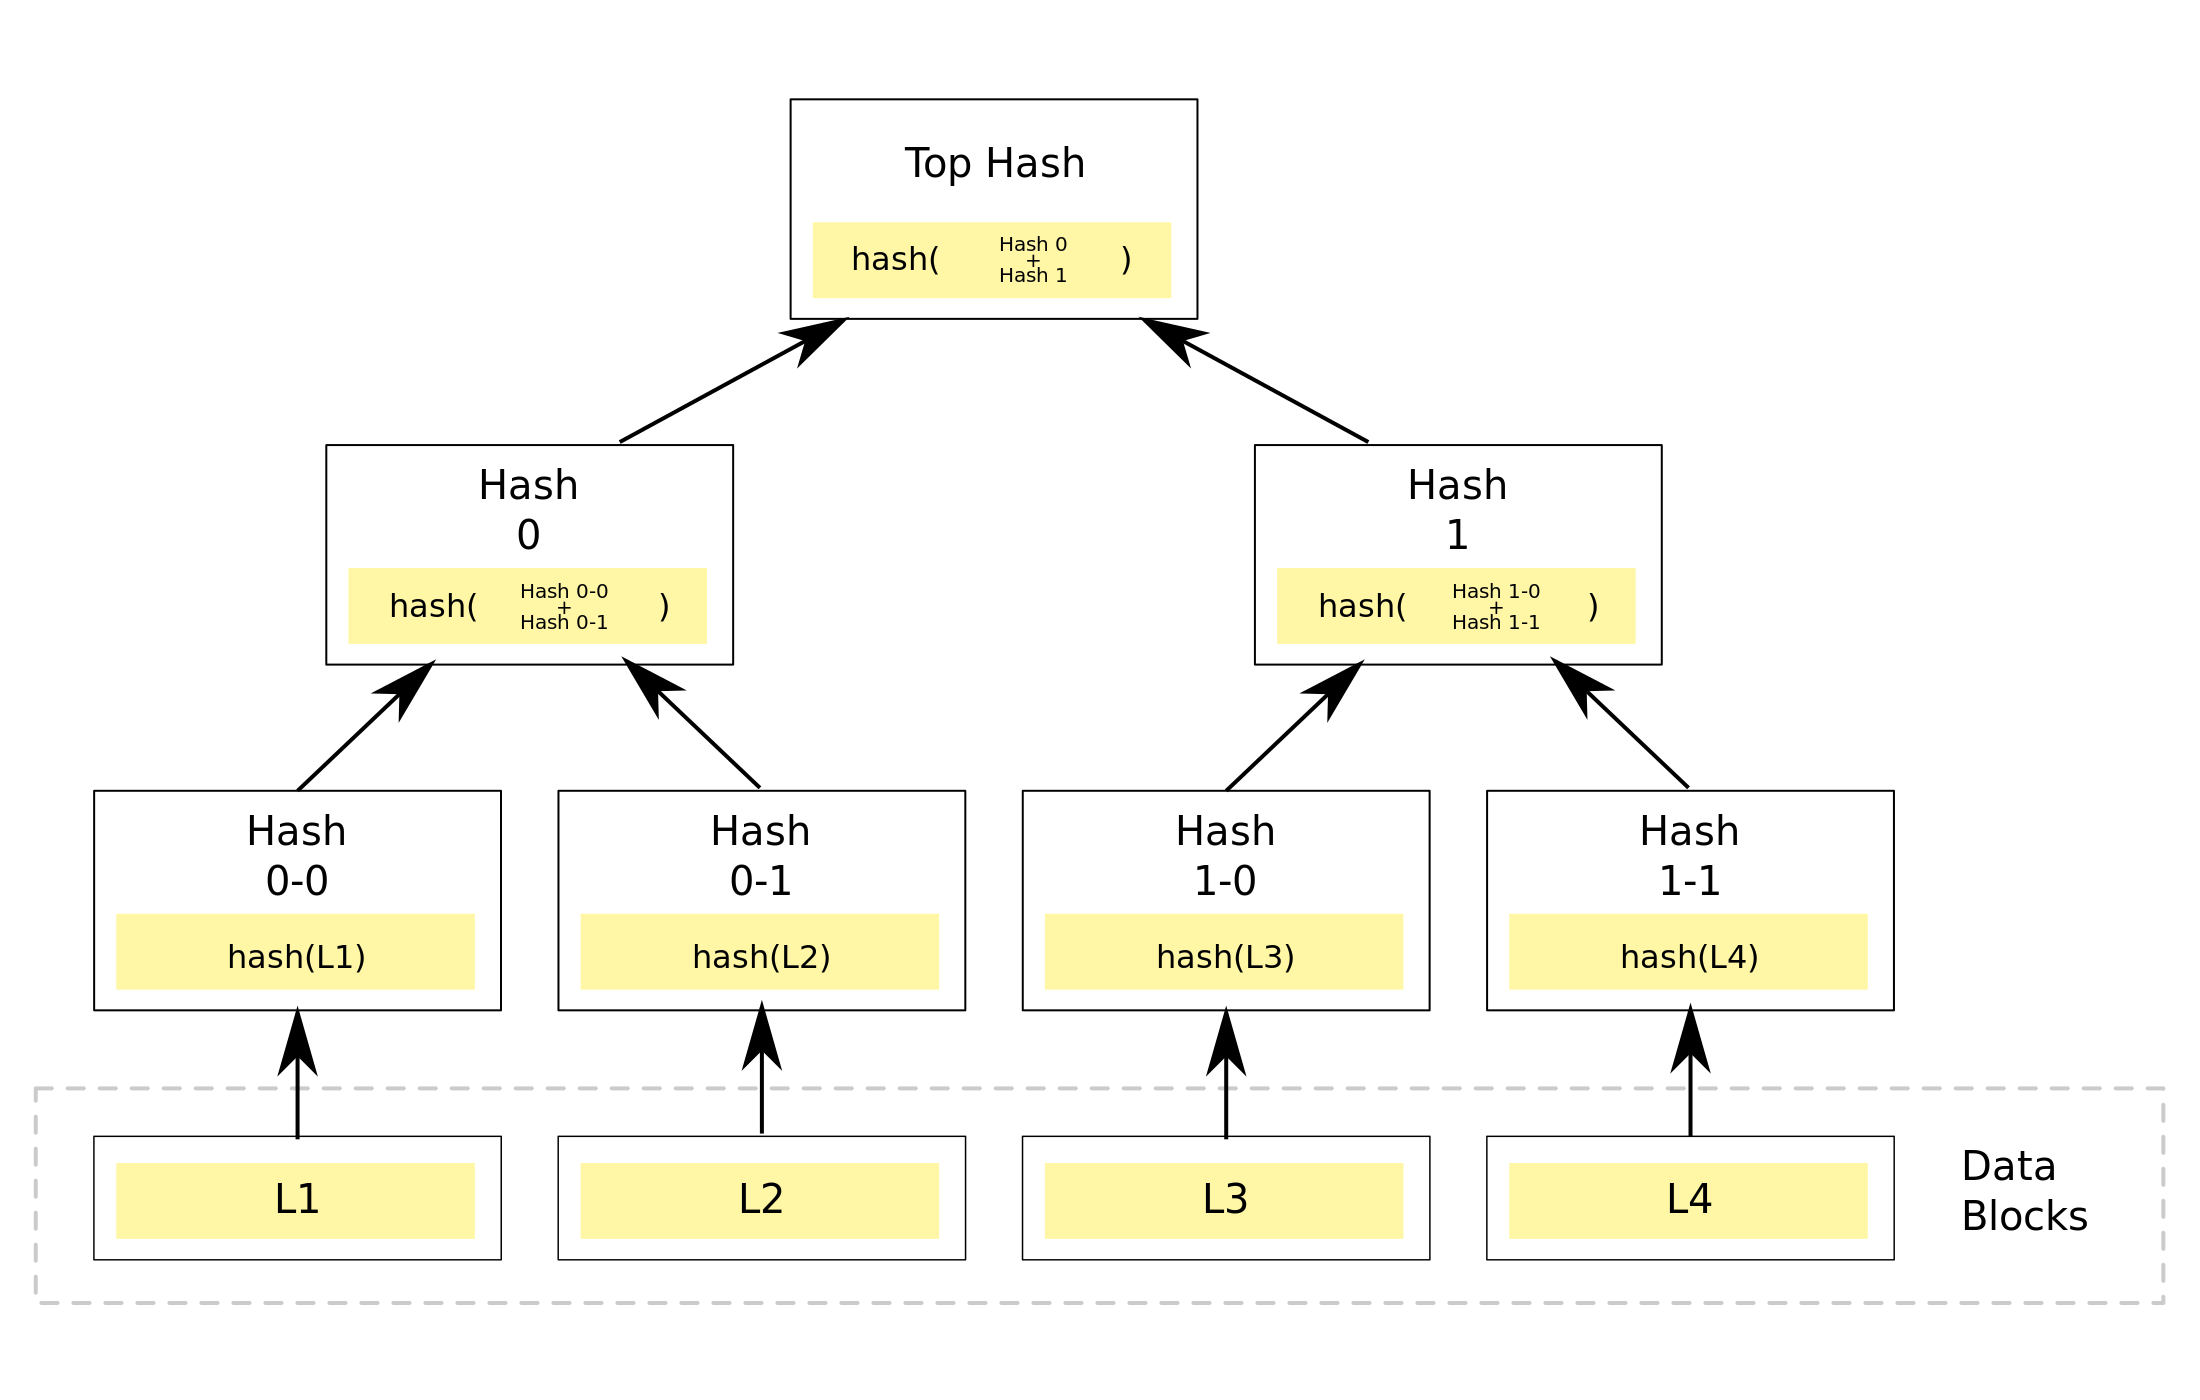
\includegraphics[width=\textwidth]{figure/MerkleTree.png}
  \begin{minipage}{\textwidth}
  \caption[Merkle Tree 示意图]{Merkle Tree 示意图\footnotemark}%
  \label{fig:merkle-tree}
  \end{minipage}
\end{figure}

\footnotetext{来源:\url{https://commons.wikimedia.org/wiki/File:Hash\_Tree.svg}}

Merkle Tree 的根节点包含了根哈希,在通过 P2P 网络下载数据时,首先会从可信
源处下载根哈希。当根哈希获取之后,就可以从其他的不可信源处获取其他的数据。
Merkle Tree 与哈希链相比的好处就是哈希树不必在所有数据都获取之后才能够校验
正确性,当哈希树的一个子树获取之后就可以对子树进行校验,这样能够加快校验,
尽早知道数据的错误性。

在图 \ref{fig:merkle-tree} 中,若目前已经获得了 hash 0--0 以及 hash 1,此时
又获得了 L2,那么现在 L2 的正确性就能够知道:通过对 L2 进行哈希获得 hash 0--1,
之后根据 hash 0--1 和 hash 0--0 来获得 hash 0,再与 hash 1 一起进行哈希,并把
结果与根哈希进行对比,如果一致则说明 L2 是正确的。能够看到,在这种情况下即使
L1,L3 和 L4 都没有下载完,仍然可以校验 L2 的正确性。如果下载过程中发现某块
的校验信息不对,就会立刻开始从其他源获取对应的块,直到校验成功。

\section{Merkle Tree 实现}

\subsection{语言与环境}

在本课程中 Merkle Tree 使用 C++ 语言实现,使用 C++ 模板来提供不同保存数据
类型的支持。项目使用 CMake 作为编译工具链,使用了 crypto++ 库\footnote{\url{https://www.cryptopp.com}}
来生成数据默认的
SHA256 哈希。

该项目代码可在 \url{https://github.com/cs-qyzhang/MerkleTree} 获取。项目中
文件及其作用为:

\dirtree{%
  .1 MerkleTree.
  .2 doc/\DTcomment{文档文件夹}.
  .3 report.tex\DTcomment{本报告 \LaTeX 源码}.
  .3 mydoc.cls\DTcomment{本报告 \LaTeX 文档类}.
  .3 report.pdf\DTcomment{本报告 PDF 文件}.
  .3 *.txt\DTcomment{测试结果}.
  .3 *.gnu\DTcomment{gnuplot 绘图程序}.
  .2 include/\DTcomment{Merkle Tree 源码文件夹}.
  .3 merkletree.h\DTcomment{Merkle Tree 定义与实现}.
  .3 bloomfilter.h\DTcomment{布隆过滤器定义与实现}.
  .2 tests/\DTcomment{测试程序文件夹}.
  .3 benchmark.cc\DTcomment{测试文件}.
  .2 CMakeLists.txt\DTcomment{CMake 文件}.
  .2 LICENSE\DTcomment{GNU GPL-3.0 许可文件}.
  .2 README.md\DTcomment{自述文件}.
}

\vfill

\subsection{关键数据结构定义}

\subsubsection{哈希值结构}

为了支持不同的哈希函数以及哈希值大小,将数据的哈希值结构作为 Merkle Tree
模板的参数。默认情况下 Merkle Tree 使用 \code{std::string} 作为数据类型,
\code{SHA256Hash} 作为哈希值结构。\code{SHA256Hash} 结构使用 SHA256 作为
哈希函数,故哈希值的大小为 32 字节。\code{SHA256} 哈希定义了多个构造函数
方便使用,还定义了 \code{==} 操作符来进行哈希值的比较。

\code{SHA256Hash} 函数的定义如下所示。

\begin{codes}{C++}
typedef unsigned char byte;
const int sha256_size = 32;

struct SHA256Hash {
  byte hash_val[sha256_size];

  SHA256Hash(const std::string& data);
  SHA256Hash(std::string* data);
  SHA256Hash(const SHA256Hash& a);
  SHA256Hash(const SHA256Hash& a, const SHA256Hash& b);
  bool operator==(const SHA256Hash& a) const;
};
\end{codes}

\subsubsection{Merkle Tree 类}

使用模板定义了 \code{MerkleTree} 类。该模板有两个参数,第一个参数是数据的类型,
第二个参数是数据哈希值的类型。在默认情况下数据类型为 \code{std::string},数据
哈希值的类型为 \code{SHA256Hash}。

\code{MerkleTree} 的节点类型为 \code{MerkleTree::Node}。节点有 \code{left}
和 \code{right} 两个成员作为其子树。当节点为叶子节点时,\code{left} 指针为
\code{nullptr}。为了使数据结构更紧凑,使用了 union 来定义 \code{right} 子树
和叶子节点的数据 \code{data}。节点还有 \code{hash} 成员来保存哈希值,当节点
为中间节点时 \code{hash} 表示子节点哈希值字符串拼接后所对应的哈希值;当节点
为叶子节点时 \code{hash} 表示叶子节点数据的哈希值。

\code{MerkleTree} 是从数据的 \code{std::vector} 转换而来的。在构造 \code{MerkleTree}
的过程中,是从下往上依次构造,直到根节点构建成功为止。具体的构造实现在
函数 \code{BuildFromVector()} 中。

函数 \code{Verify()} 用于校验 Merkle Tree 的正确性,为了实现简单,这里的
校验只是从根哈希开始依次向下校验,若校验成功则返回 \code{true},否则
返回 \code{false}。

函数 \code{Exist()} 用于判断指定的数据块是否位于 Merkle Tree 中。在判断时,会
类似二叉树查找那样递归进行,先查左子树,再查右子树。

\code{MerkleTree} 的定义如下所示。

\begin{codes}{C++}
template< typename T = std::string, typename Hash = SHA256Hash >
class MerkleTree {
 public:
  MerkleTree();
  MerkleTree(const std::vector<T*>& data);
  void BuildFromVector(const std::vector<T*>& data);
  size_t LeafSize() const;
  int Level() const;
  bool Exist(T* data) const;
  bool Verify() const;

 private:
  struct Node {
    Node*  left;    // nullptr if is leaf
    union {
      Node*  right;
      T*     data;
    };
    Hash hash;

    bool IsLeaf() const { return left == nullptr; }
  };

  Node*     root_;    // root of tree
  size_t    nr_leaf_; // data block count
  int       level_;   // tree depth
};
\end{codes}

\section{布隆过滤器优化}

在实现中能够看到,Merkle Tree 在查找某一块数据时,因为 Merkle Tree 没有
对数据进行排序,需要遍历整个树。当数据量较大时,为了查找一个数据而遍历
整个树就会变得十分费时。

为了加快数据的定位,一个简单的优化方式是为每一个节点增加一个布隆过滤器,
在查找时就可以根据布隆过滤器来大概判断某个子树中是否可能存在,如果一定
不存在则无需去查找该子树,这样就能够减少定位的时间。

布隆过滤器在建立 Merkle Tree 的过程中同步进行。在叶子节点,布隆过滤器
只包含一个数据,也就是叶子节点指向的数据块。在中间节点,某一个节点的
布隆过滤器由其左子树和右子树构成。由于布隆过滤器通过一些标记来记录包含
哪些数据,而对于一个节点来说,其包含的数据是左子树的数据加上右子树的
数据,故其布隆过滤器的标记应该是左子树布隆过滤器和右子树布隆过滤器之``和'',
由于布隆过滤器一般采用位图来实现,所以实际的操作是左右两个子树位图的
或运算。

在加入了布隆过滤器之后,数据块的校验和定位就可以先通过布隆过滤器进行判断,
如果布隆过滤器测试为假,则说明该数据块一定不存在该节点为根节点的子树中。

布隆过滤器的实现在 \code{include/bloomfilter.h} 中,其定义如下:

\begin{codes}{C++}
template<typename T, size_t bitset_len = 10000>
class BloomFilter {
 public:
  BloomFilter() = default;
  BloomFilter(const BloomFilter& a) { set_ = a.set_; }

  BloomFilter(const std::vector<T*> data) {
    for (auto& d : data)
      Add(d);
  }

  BloomFilter(const BloomFilter& a, const BloomFilter& b) {
    set_ = a.set_ | b.set_;
  }

  void Add(T* data);
  bool MaybeExist(T* data) const;

 private:
  std::bitset<bitset_len> set_;
};
\end{codes}

\code{BloomFilter} 模板有两个参数,第一个参数是数据块的类型,第二个参数是
位图的长度。能够看到,\code{BloomFilter} 能够从两个 \code{BloomFilter}
快速构建,新的位图是两个位图的或。

为了使用布隆过滤器,\code{MerkleTree::Node} 结构新增了一个 \code{filter}
成员,\code{MerkleTree} 新增了函数 \code{ExistUseBloom} 来用布隆过滤器
加快查找。

\section{测试}

\subsection{测试环境}

\begin{itemize}
  \item \textbf{CPU:} Intel(R) Core(TM) i5-10210U CPU @ 1.60GHz
  \item \textbf{DRAM:} 16 GB
  \item \textbf{OS:} Ubuntu 20.04
  \item \textbf{Kernel:} 5.4.0
  \item \textbf{Compiler:} GCC 9.3.0
\end{itemize}

\subsection{Merkle Tree 构建时间及空间使用测试}

首先对 Merkle Tree 的构建时间及空间使用进行测试,测试时数据为 \code{std::string}
类型,节点没有使用布隆过滤器。分别在不同数据量下进行测试,记录下测试
得到的构建时间、树的高度、空间使用(不包含数据块占用的空间)等,测试
获得的数据如表 \ref{tab:build-time} 所示,数据在 logscale 坐标下的折线图
如图 \ref{fig:build-time} 所示。

能够看到,1ms 平均能够构建 801 个数据,1 MB 空间能够保存 10922 个数据。
随着数据量的增加,树的层数逐渐增高,但即使是 10M 数据树的层数也只有 25。

\begin{figure}[htbp]
  \centering
  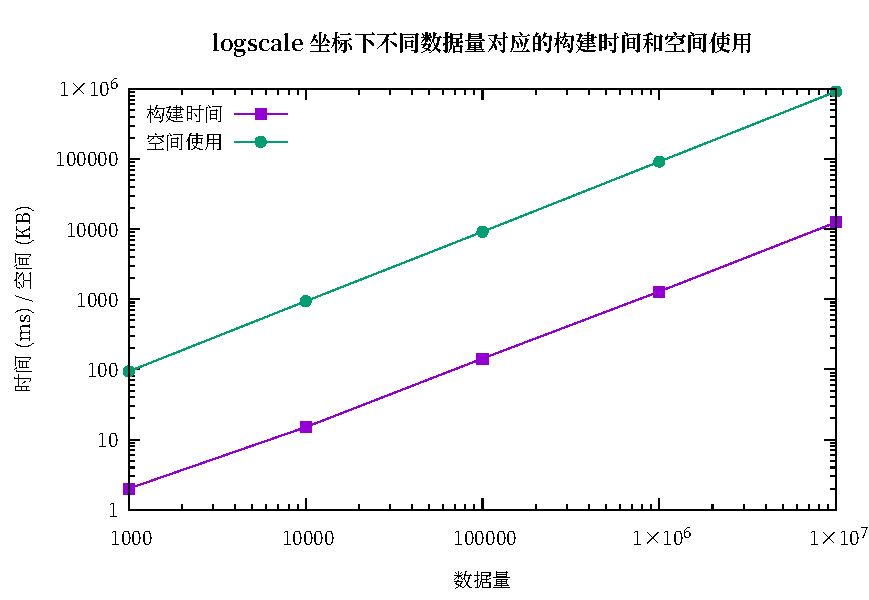
\includegraphics{figure/build-time.pdf}
  \caption{logscale 坐标下不同数据量对应的构建时间和空间使用}%
  \label{fig:build-time}
\end{figure}

\begin{table}[htbp]
  \centering
  \caption{不同数据量对应的构建时间和空间占用}%
  \label{tab:build-time}

  \vspace{10pt}
  \begin{tabular}{lrrr}
    \toprule
    \textbf{数据块数} & \textbf{构建时间} & \textbf{树的层数} & \textbf{空间使用} \\
    \midrule
    1000              & 2ms               & 11                & 93.80 KB  \\
    10,000            & 15ms              & 15                & 937.73 KB \\
    100,000           & 143ms             & 18                & 9.16 MB   \\
    1000,000          & 1,289ms           & 21                & 91.55 MB  \\
    10,000,000        & 12,482ms          & 25                & 915.53 MB \\
    \bottomrule
  \end{tabular}
\end{table}

\subsection{布隆过滤器优化对比测试}

为了体现布隆过滤器的优势,分别在节点有布隆过滤器以及节点无布隆过滤器两种
情况下对数据的定位速度进行测试。节点有无布隆过滤器可以通过 \code{BLOOM}
宏的有无进行条件编译。

\subsubsection{假数据比例对性能的影响}

首先在不同``假''数据比例下进行测试,这里的``假''数据指的是不包含在 Merkle
Tree 中的数据。当假数据比例为 0 时代表测试数据都在 Merkle Tree 中;当假数据
比例为 1 时代表测试数据都不在 Merkle Tree 中。测试时记录下 1K 数据的定位时间,
具体的测试结果如图 \ref{fig:false-percent} 和表 \ref{tab:false-percent} 所示。

能够看到,随着假数据比例的提升,没有布隆过滤器的 Merkle Tree 每 1K
数据的定位时间呈线性增加,这是因为当数据位于 Merkle Tree 时,平均需要
查找 $\frac{n}{2}$ 个节点,而当数据没有位于 Merkle Tree 时,需要对所有
的 $n$ 个数据都要进行对比。

而对于有布隆过滤器的 Merkle Tree 来说,假数据的比例对性能的影响不大,
这是因为布隆过滤器能够直接判断出一些假数据不存在于 Merkle Tree 中,
不需要对所有 $n$ 个数据进行对比查询。

\subsubsection{布隆过滤器比特数量对性能的影响}

布隆过滤器的位图大小越大使用的空间越大,性能越好,所以这里使用不同的位图
大小来测试性能。测试时位图中比特的数量是与总数据量相关的,测试时分别取位图
比特与总数据量的不同比例进行测试,统计每 1K 数据的定位时间以及 Merkle Tree
的空间使用(不包含数据块)。当位图比特与总数据量之比为 0 时意味着不使用布隆
过滤器。测试结果如图 \ref{fig:bloom-test} 和表 \ref{tab:bloom-test} 所示。

能够看到,随着位图大小的增加,空间使用线性增加,而定位时间则以类似于 $\frac{1}{x}$
函数的形式逐渐减少。在位图与数据的比例为 0.1 附近效果较好。

\begin{table}[htbp]
  \centering
  \caption{不同假数据比例下有无布隆过滤器测试 1K 数据使用的时间}%
  \label{tab:false-percent}

  \vspace{10pt}
  \begin{tabular}{crr}
    \toprule
    \textbf{假数据比例} & \textbf{有布隆过滤器时间} & \textbf{无布隆过滤器时间} \\
    \midrule
    0.00 & 67.20ms  & 5.60ms \\
    0.05 & 70.59ms  & 5.80ms \\
    0.10 & 74.25ms  & 6.39ms \\
    0.20 & 79.84ms  & 6.48ms \\
    0.30 & 87.57ms  & 6.86ms \\
    0.40 & 94.20ms  & 7.26ms \\
    0.50 & 100.40ms & 7.40ms \\
    0.60 & 106.96ms & 7.52ms \\
    0.70 & 111.48ms & 7.98ms \\
    0.80 & 120.70ms & 8.24ms \\
    0.90 & 125.32ms & 8.58ms \\
    1.00 & 134.70ms & 8.90ms \\
    \bottomrule
  \end{tabular}
\end{table}

\begin{figure}[htbp]
  \centering
  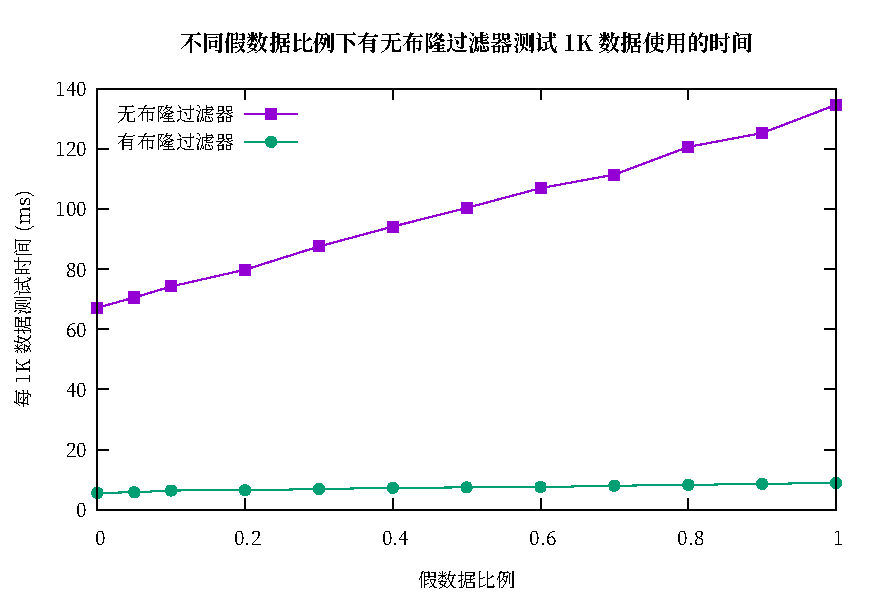
\includegraphics{figure/benchmark-false-percent.pdf}
  \caption{不同假数据比例下有无布隆过滤器测试 1K 数据使用的时间}%
  \label{fig:false-percent}
\end{figure}

\begin{table}[htbp]
  \centering
  \caption{布隆过滤器在位图与数据不同比例下定位时间与空间使用}%
  \label{tab:bloom-test}

  \vspace{10pt}
  \begin{tabular}{crr}
    \toprule
    \textbf{位图与数据量之比} & \textbf{每 1K 测试时间} & \textbf{空间使用} \\
    \midrule
    0.0  & 116.43ms & 0.93 KB  \\
    0.01 & 41.43ms  & 1.22 KB  \\
    0.02 & 25.40ms  & 1.53 KB  \\
    0.03 & 17.93ms  & 1.68 KB  \\
    0.04 & 15.53ms  & 1.98 KB  \\
    0.06 & 11.53ms  & 2.44 KB  \\
    0.08 & 9.07ms   & 2.90 KB  \\
    0.10 & 7.97ms   & 3.36 KB  \\
    0.20 & 5.37ms   & 5.80 KB  \\
    0.30 & 4.30ms   & 8.09 KB  \\
    0.40 & 3.57ms   & 10.53 KB \\
    0.60 & 3.10ms   & 15.26 KB \\
    0.80 & 2.67ms   & 19.99 KB \\
    1.00 & 2.40ms   & 24.88 KB \\
    1.20 & 2.20ms   & 29.61 KB \\
    1.50 & 2.07ms   & 36.78 KB \\
    2.00 & 1.93ms   & 48.69 KB \\
    \bottomrule
  \end{tabular}
\end{table}

\begin{figure}[htbp]
  \centering
  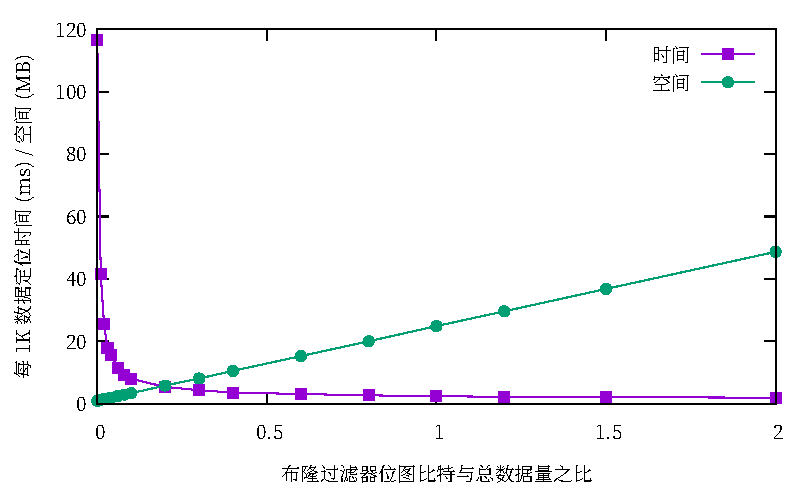
\includegraphics{figure/benchmark-bloom.pdf}
  \caption{布隆过滤器在位图与数据不同比例下定位时间与空间使用}%
  \label{fig:bloom-test}
\end{figure}

\clearpage

\end{document}